 \documentclass[12pt]{scrartcl}
\usepackage[sexy]{ekesh}
\usepackage[noend]{algpseudocode}
\usepackage{answers}
\usepackage{array}
\usepackage{tikz}
\newenvironment{allintypewriter}{\ttfamily}{\par}
\usepackage{listings}
\usepackage{xcolor}
\usetikzlibrary{arrows.meta}
\usepackage{color}
\usepackage{mathtools}
\newcommand{\U}{\mathcal{U}}
\newcommand{\E}{\mathbb{E}}
\usetikzlibrary{arrows}
\Newassociation{hint}{hintitem}{all-hints}
\renewcommand{\solutionextension}{out}
\renewenvironment{hintitem}[1]{\item[\bfseries #1.]}{}
\renewcommand{\O}{\mathcal{O}}
\declaretheorem[style=thmbluebox,name={Chinese Remainder Theorem}]{CRT}
\renewcommand{\theCRT}{\Alph{CRT}}
\setlength\parindent{0pt}
\usepackage{sansmath}
\usepackage{pgfplots}
\usetikzlibrary{automata}
\usetikzlibrary{positioning}  %                 ...positioning nodes
\usetikzlibrary{arrows}       %                 ...customizing arrows
\newcommand{\eqdef}{=\vcentcolon}
\usepackage[top=3cm,left=3cm,right=3cm,bottom=3cm]{geometry}
\newcommand{\mref}[3][red]{\hypersetup{linkcolor=#1}\cref{#2}{#3}\hypersetup{linkcolor=blue}}%<<<changed

\tikzset{node distance=4.5cm, % Minimum distance between two nodes. Change if necessary.
         every state/.style={ % Sets the properties for each state
           semithick,
           fill=cyan!40},
         initial text={},     % No label on start arrow
         double distance=4pt, % Adjust appearance of accept states
         every edge/.style={  % Sets the properties for each transition
         draw,
           ->,>=stealth',     % Makes edges directed with bold arrowheads
           auto,
           semithick}}


% Start of document.
\newcommand{\sep}{\hspace*{.5em}}


\begin{document}
\title{Design and Analysis of Algorithms}
\author{Ekesh Kumar\thanks{Email: \mailto{ekumar1@terpmail.umd.edu}}}
\date{\today}

\definecolor{dkgreen}{rgb}{0,0.6,0}
\definecolor{gray}{rgb}{0.5,0.5,0.5}
\definecolor{mauve}{rgb}{0.58,0,0.82}

\lstset{frame=tb,
  aboveskip=3mm,
  belowskip=3mm,
  showstringspaces=false,
  columns=flexible,
  basicstyle={\small\ttfamily},
  numbers=none,
  numberstyle=\tiny\color{gray},
  keywordstyle=\color{blue},
  commentstyle=\color{dkgreen},
  stringstyle=\color{mauve},
  breaklines=true,
  breakatwhitespace=true,
  tabsize=3
}

\maketitle
These are my course notes for CMSC 451: Design and Analysis of Algorithms, taught by Professor Clyde Kruskal. Gaps in lecture material are filled in with CLRS and Kleinberg \& Tardos. Please send corrections to \url{ekumar1@terpmail.umd.edu}.

\tableofcontents


\newpage

\section{Tuesday, January 28, 2020}

\subsection{Introduction}

This is CMSC $451$: Design and Analysis of Algorithms. We will cover graphs, greedy algorithms, divide and conquer algorithms, dynamic programming, network flows, NP-completeness, and approximation algorithms.


\begin{itemize}
    \item Homeworks are due every other Friday or so; NP-homeworks are typically due every other Wednesday.
    \item There is a $25\%$ penalty on late homeworks, and there's one get-out-of-jail free card for each type of homework.
\end{itemize}

\subsection{Stable Marriage Problem}

As an introduction to this course, we'll discuss the \vocab{stable marriage problem}, which is stated as follows:

\begin{quote}
    Given a set of $n$ men and $n$ women, match each man with a woman in such a way that the matching is \textit{stable}.
\end{quote}

What do we mean when we call a matching is ``stable"? We call a matching \textit{unstable} if there exists some man $M$ who prefers a woman $W$ over the woman he is married to, and $W$ also prefers $M$ over the man she is currently married to. \\



In order to better understand the problem, let's look at the $n = 2$ case. Call the two men $M_1$ and $M_2$, and call the two women $W_1$ and $W_2$.

\begin{itemize}
    \item First suppose $M_1$ prefers $W_1$ over $W_2$ and $W_1$ prefers $M_1$ over $M_2$. Also, suppose that $M_2$ prefers $W_2$ over $W_1$ and $W_2$ prefers $M_2$, then 
    \item If both $W_1$ and $W_2$ prefer $M_1$ over $M_2$, and both $M_1$ and $M_2$ prefer $W_1$ over $W_2$, then it's still easy to see what will happen: $M_i$ will always match with $W_i$.
    \item Now let's say $M_1$ prefers $W_1$ to $W_2$, $M_2$ prefers $W_2$ to $W_1$, $W_1$ prefers $M_2$ to $M_1$, and $W_2$ prefers $M_1$ to $M_2$. In this case, the two men rank different women first, and the two women rank different men first. However, the men's preferences ``clash" with the women's preferences. One solution to this problem is to match $M_1$ with $W_1$ and $M_2$ with $W_2$. This is stable since both men get their top preference even though the two women are unhappy.
\end{itemize}

The solution to the problem starts to get a lot more complicated when the people's preferences do not exhibit any pattern. So how do we solve this problem in the general case? We can use the \vocab{Gale-Shapley algorithm}. Before discussing this algorithm, however, we can make the following observations about this problem:

\begin{itemize}
    \item Each of the $n$ men and $M$ woman are initially unmarried. If an unmarried man $M$ chooses the woman $W$ who is ranked highest on their list, then we cannot immediately conclude whether we can match $M$ and $w$ in our final matching.This is clearly the case since if we later find out about some other man $M_2$ who prefers $W$ over any other woman, $W$ may choose $M_2$ if she likes him more than $M$. However, we cannot immediately rule out  $M$ being matched to $W$ either since a man like $M_2$ may not ever come. 
    \item Just because everyone isn't happy doesn't mean a matching isn't stable. Some people might be unhappy, but there might not be anything they can do about it (if nobody wants to switch).
\end{itemize}


Moreover, we introduce the notion of a man \textit{proposing} to a woman, which a woman can either accept or reject. If she is already engaged and accepts a proposal, then her existing engagement breaks off (the previous man becomes unengaged).  \\


Now that we've introduced these basic ideas, we can now present the algorithm:


\vspace{1em}
\hline
\vspace{1em}

\begin{allintypewriter}
\# Input: A list of n men and n women to be matched. 

\hspace{0.5cm} 

\# Output: A valid stable matching.


\hspace{0.5cm}


stable\_matching \string{ 

\hspace{0.5cm} set each man and each woman to "free"

\hspace{0.5cm} while there exists a man m who still has a woman w to propose to \string{

\hspace{1cm} let w be the highest ranked woman m hasn't proposed to. 

\hspace{0cm}

\hspace{1cm} if w is free \string{ 

\hspace{1.5cm} (m, w) become engaged 

\hspace{1cm} \string} else \string{

\hspace{1.5cm} let m' be the man w is currently engaged to.

\hspace{1.5cm} if w prefers m' to m \string{ 

\hspace{2cm} (m', w) remain engaged. 

\hspace{1.5cm} \string} else \string{

\hspace{2cm} (m, w) become engaged and m' loses his partner.

\hspace{1.5cm} \string}

\hspace{1cm} \string}

\hspace{0.5cm} \string}

\string}

\end{allintypewriter}
\vspace{1em}
\hline
\vspace{1em}


\begin{proposition}
The Gale-Shapley algorithm terminates in $\mathcal{O}(n^2)$ time. 
\end{proposition}
\begin{proof}
In the worst case, $n$ men end up proposing to $n$ women. The act of proposing to another person is a constant-time operation. Thus, the $\mathcal{O}(n^2)$ runtime is clear.
\end{proof}%
\newpage
\section{Thursday, January 30, 2020}

\subsection{Optimality and Correctness of Gale-Shapley}


Last time, we introduced the Gale-Shapley algorithm to find a stable matching. Today, we'll prove that the algorithm is correct (i.e. it never produces an unstable matching), and it is optimal for men (i.e. the men always end up for their preferred choice). \\

First, we'll show that the algorithm is correct: \\

\begin{proposition}
The matching generated by the Gale-Shapley algorithm is never an unstable matching.  
\end{proposition}

\begin{proof}
Suppose, for the sake of contradiction, that $m$ and $w$ prefer each other over their current partner in the matching generated by the Gale-Shapley algorithm. This can happen either if $m$ never proposed to $w$, or if $m$ proposed to $w$ and $w$ rejected $m$. In the former case, $m$ must prefer his partner to $w$, which implies that $m$ and $w$ do not form an unstable pair. In the latter case, $w$ prefers her partner to $m$, which also implies $m$ and $w$ don't form an unstable pair. Thus, we arrive at a contradiction. 
\end{proof}

Next, we'll prove that the algorithm is optimal for men. However, before presenting the proof, observe that it is not too hard to see intuitively that the algorithm ``favors" the men. Since the men are doing all of the proposing and the women can only do the deciding, it turns out that the men always ends up with their most preferred choice (as long as the matching remains stable).

\begin{proposition}
The matching generated by the Gale-Shapley algorithm gives men their most preferred woman possible without contradicting stability. 
\end{proposition}

\begin{proof}
 \\



To see why this is true, let $A$ be the matching generated by the men-proposing algorithm, and suppose there exists some other matching $B$ that is better for at least one man, say $m_0$. If $m_0$ is matched in $B$ to $w_1$ which he prefers to his match in $A$, then in $A$, $m_0$ must have proposed to $w_1$ and $w_1$ must have rejected him. This can only happen if $w_1$ rejected him in favor of some other man --- call him $m_2$. This means that in $B$, $w_1$ is matched to $m_0$ but she prefers $m_2$ to $m_0$. Since $B$ is stable, $m_2$ must be matched to some woman that he prefers to $w_1$; say $w_3$. This means that in $A$, $m_2$ proposed to $w_3$ before proposing to $w_1$, and this means that $w_3$ rejected him. Since we can perform similar considerations, we end up tracing a ``cycle of rejections" due to the finiteness of the sets $A$ and $B$. 
\end{proof}



% Feb
\section{Tuesday, February 4, 2020}

Today, we'll recap graph terminology and elementary graph algorithms.

\subsection{Graph Terminology}

\begin{definition}
A \vocab{graph} $G = (V, E)$ is defined by a set of vertices $V$ and a set of edges $E$.
\end{definition}

The number of vertices in the graph, $|V|$, is the \vocab{order} of the graph, and the number of edges in the graph, $|E|$, is the \vocab{size} of the graph. Typically, we reserve the letter $n$ for the order of a graph, and we reserve $m$ for the size of a graph. 
\begin{definition}
We say a graph is \vocab{directed} if its edges can only be traversed in one direction. Otherwise, we say the graph is  \vocab{undirected}.
\end{definition}


\begin{definition}
A graph is called \vocab{simple} if it's an undirected graph without any loops (edges that start and end at the same vertex).
\end{definition}

\begin{definition}
A graph is \vocab{connected} if for every pair of vertices $u, v$, there exists a path between $u$ and $v$.
\end{definition}


\subsection{Graph Representations}

There are two primary ways in which we can represent graphs: \vocab{adjacency matrices} and \vocab{adjacency lists}. \\


An adjacency matrix is an $n\times n$ matrix \verb!A! in which \verb!A[u][v]! is equal to $1$ if the edge $(u, v)$ exists in the graph; otherwise, \verb!A[u][v]! is equal to $0$. Note that the adjacency matrix is symmetric if and only if the graph is undirected. \\

On the other hand, an adjacency list is a list of $|V|$ lists, one for each vertex. For each vertex $u \in V$, the adjacency list \verb!Adj[u]! contains all vertices $v$ for which there exists an edge $(u, v)$ in $E$. In other words, \verb!Adj[u]! contains all of the vertices adjacent to $u$ in $G$.  


Each graph representation has its advantages and disadvantages in terms of runtime. This is summarized by the table below.

\begin{figure}[h]
\centering
\begin{tabular}{ | m{2cm} | m{4cm}| m{4cm} | } 
\hline
 & \textsc{Adjacency List} & \textsc{Adjacency Matrix} \\ 
\hline
Storage  & $\mathcal{O}(n + m)$ & $\O(n^2)$ \\ 
\hline
Add vertex & $\mathcal{O}(1)$ & $\O(n^2)$ \\ 
\hline
Add edge & $\mathcal{O}(1)$ & $\O(1)$ \\ 
\hline
Remove vertex & $\mathcal{O}(n + m)$ & $\O(n^2)$ \\ 
\hline
Remove edge & $\mathcal{O}(m)$ & $\O(1)$ \\ 
\hline
\end{tabular}
\caption{Adjacency Matrix vs Adjacency List}
\end{figure}

An explanation of these runtimes are provided below:

\begin{itemize}
    \item An adjacency list requires $\O(n + m)$ since there are $n$ lists inside of the adjacency list. Now for each vertex $v_i$, there are $\text{deg}(v_i)$ vertices in the $i^{\text{th}}$ adjacency list. Since $\sum_{i} \text{deg}(v_i) = \O(m)$, we conclude that the adjacency list representation of a graph requires $\O(n + m)$ space. On the other hand, the adjacency matrix representation of a graph requires $\mathcal{O}(n^2)$ space since we are storing an $n\times n$ matrix. 
    \item We can add a vertex in constant time in an adjacency list by simply inserting a new list into the adjacency list. On the other hand, to insert a new vertex in an adjacency matrix, we need to increase the dimensions of the adjacency matrix from $n\times n$ to $(n + 1) \times (n + 1)$. This requires $\mathcal{O}(n^2)$ time since we need to copy over the old matrix to a new matrix.
    \item We can insert an edge $(u, v)$ into an adjacency list in constant time by simply appending $v$ to the end of $u$'s adjacency list (and $u$ to the end of $v$'s adjacency list if the graph is undirected). Similarly, we can insert an edge in an adjacency matrix in constant time by setting \verb!A[u][v]! to $1$ (and also seting \verb!A[v][u]! to $1$ if the graph is undirected). 
    \item Removing a vertex requires $\mathcal{O}(n + m)$ time in an adjacency list since we need to traverse the entire adjacency list and remove any incoming our outgoing edges to the vertex being removed. Similarly, this operation takes $\O(n^2)$ time in an adjacency matrix since we need to traverse the entire matrix to remove incoming and outgoing edges.
    \item Removing an edge $(u, v)$ requires $\mathcal{O}(m)$ time in an adjacency matrix since we only need to search the adjacency lists of $u$ and $v$ (in the worst case, these vertices have all $m$ edges in their adjacency list). On the other hand, this operation takes constant time in an adjacency matrix since we're just setting \verb!A[u][v]! to $0$.
\end{itemize}


\subsection{Graph Traversal}

Before discussing recapping the two primary types of graph traversal, we will introduce some more terminology. \\

\begin{definition}
A \vocab{connected component} of a graph is a maximially connected subgraph of $G$. Each vertex belongs to one connected component as does each edge.
\end{definition}

There are two primary ways in which we can traverse graphs: using \vocab{breadth-first search} or \vocab{depth-first search}. These two methods of graph traversal are very similar, and they allow us to explore every vertex in a connected components of a graph. 


\begin{enumerate}
    \item Breadth-first search starts at some source vertex $v$ and all vertices with distance $k$ away from $v$ before visiting vertices with distance $k + 1$ from $v$. This algorithm is typically implemented using a queue, and it can be used to find the shortest path (measured by the number of edges) from the source vertex.
    \item Depth-first search starts from a source vertex and keeps on going outward until we cannot proceed any further. We must subsequently backtrack and begin performing the depth-first search algorithm again.  This algorithm is typically implemented using a stack, whether it be the data structure or the function call stack.
\end{enumerate}

Both of these algorithms run in $\O(n^2)$ time on an adjacency matrix and $\O(n + m)$ time on an adjacency list. \\

Since breadth-first search and depth-first search are guaranteed to visit all of the vertices in the same connected component as the starting vertex, we can easily write an algorithm that counts the number of connected components in a graph. \\

Some C++ code is provided below.

\begin{lstlisting}
/* visited[] is a global Boolean array. */
/* AdjList is a global vector of vectors. */
void dfs(int v) {
    visited[v] = true;
    for (int i = 0; i < AdjList[v].size(); i++) {
        int u = AdjList[v][i];
        if (!visited[u]) {
            dfs(v);
        }
    }
}

int main(void) {
    /* Assume AdjList and other variables have been declared. */
    int numCC = 0;
    for (int i = 0; i < num_vertices; i++) {
        if (!visited[i]) {
            numCC = numCC + 1;
            dfs(i);
        }
    }
}
\end{lstlisting}
\newpage
\section{Thursday, February 6, 2020}

Today, we'll discuss algorithms to find articulation points and biconnected components. 

\subsection{Articulation Points}

\begin{definition}
An \vocab{articulation point} or \vocab{cut vertex} is a vertex in a graph $G = (V, E)$ whose removal (along with any incident edges) would disconnect $G$. 
\end{definition}

\begin{definition}
A graph is said to be \vocab{biconnected} if the graph not have any articulation points. 
\end{definition}

For example, consider the following graph:

\begin{figure}[h]
\centering
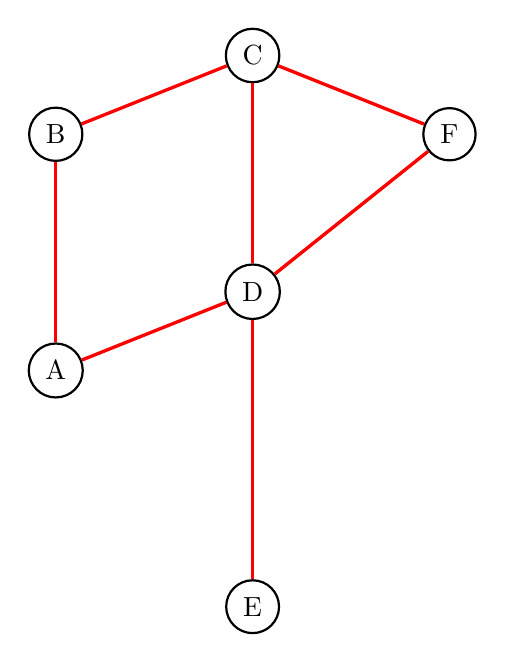
\begin{tikzpicture}
\begin{scope}[every node/.style={circle,thick,draw}]
    \node (A) at (0,0) {A};
    \node (B) at (0,3) {B};
    \node (C) at (2.5,4) {C};
    \node (D) at (2.5,1) {D};
    \node (E) at (2.5,-3) {E};
    \node (F) at (5,3) {F} ;
\end{scope}

\begin{scope}[>={Stealth[black]},
              every node/.style={fill=white,circle},
              every edge/.style={draw=red,very thick}]
    \path [-] (A) edge (B);
    \path [-] (B) edge (C);
    \path [-] (A) edge (D);
    \path [-] (D) edge (C);
    % \path [-] (A) edge (E);
    \path [-] (D) edge (E);
    \path [-] (D) edge (F);
    \path [-] (C) edge (F);
    % \path [-] (E) edge (F); 
    % \path [-] (B) edge[bend right=40] (F); 
\end{scope}
\end{tikzpicture}
\caption{A Graph with an Articulation Point}
\end{figure}

In the diagram above, Vertex $D$ is an articulation point. To see why, note that if we were to remove Vertex $D$ (and any incident edges to $D$) from the graph, then we would end up with two connected components: the first component would contain the vertices $A, B, C,$ and $F$, whereas the second component would only contain the vertex $E$. \\

Why are articulation points important? One example in which searching for articulation points is important is in the study of networks. In a network modeled by a graph, an articulation point represents a vulnerability: it is a single point whose failure would split the network into two or more components (preventing communication between the nodes in different networks). 
 \\
 
 
 How do we find an articulation points? The brute force algorithm is as follows:
 
 \begin{enumerate}
     \item Run an $\mathcal{O}(V + E)$ depth-first search or breadth-first search to count the number of connected components in the original graph $G = (V, E)$. 
     \item For each vertex $v\in V$, remove $v$ from $G$, and remove any of $v$'s incident edges. Run an $\mathcal{O}(V + E)$ depth-first search or breadth-first search again, and check if the number of connected components increases. If so, then $v$ is an articulation point. Restore $v$ and any of its incident edges.
 \end{enumerate}
 
This naive algorithm calls the depth-first search or breadth-first search algorithm $\mathcal{O}(V)$ times. Hence, it runs in $\mathcal{O}(V \times (V + E)) = \mathcal{O}(V^2 + VE)$ time. \\
 
 
While this algorithm \textit{works}, it is not as efficient as we can get. We will now describe a linear-time algorithm that runs the depth-first search algorithm just \textit{once} to identify all articulation points and bridges. This algorithm is often accredited to Hopcraft and Tarjan. \\
 
 
In this modified depth-first search, we will now maintain two numbers for each vertex $v$: \verb!dfs_num(v)! and \verb!dfs_low(v)!. The quantity \verb!dfs_num(v)! represents a label that we will assign to nodes in an increasing fashion. For instance, the vertex from which we call depth-first search would have a \verb!dfs_num! of $0$. The subsequent vertex we visit would be assigned a \verb!dfs_num! of $1$, and so on. \\
 
On the other hand, the quantity \verb!dfs_low(v)!, also known as the \vocab{low-link value} of the vertex $v$, represents the smallest \verb!dfs_num! reachable from that node while performing a depth-first (including itself). \\
 
Here's an example. Consider the following directed graph: 
  
  
\begin{figure}[h]
\centering
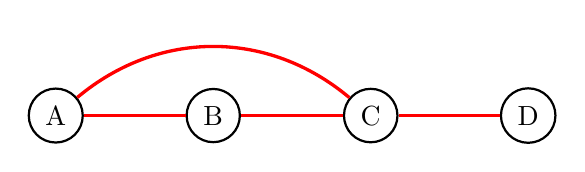
\begin{tikzpicture}
\begin{scope}[every node/.style={circle,thick,draw}]
    \node (A) at (0,0) {A};
    \node (B) at (2,0) {B};
    \node (C) at (4,0) {C};
    \node (D) at (6,0) {D};
    % \node (E) at (2.5,-3) {E};
    % \node (F) at (5,3) {F} ;
\end{scope}

\begin{scope}[>={Stealth[black]},
              every node/.style={fill=white,circle},
              every edge/.style={draw=red,very thick}]
    \path [-] (A) edge (B);
    \path [-] (B) edge (C);
    \path [-] (C) edge (D);
    \path [-] (C) edge[bend right=40] (A); 

    % \path [-] (A) edge (D);
    % \path [-] (D) edge (C);
    % \path [-] (A) edge (E);
    % \path [-] (D) edge (E);
    % \path [-] (D) edge (F);
    % \path [-] (C) edge (F);
    % \path [-] (E) edge (F); 
    % \path [-] (B) edge[bend right=40] (F); 
\end{scope}
\label{artpoint:ex}
\end{tikzpicture}
\caption{Articulation Point Example}
\end{figure}

Suppose we perform a depth-first search starting at Vertex $A$. 

\begin{itemize}
    \item Vertex $A$ will be assigned a \verb!dfs_num! of $0$ since this is the first vertex that we're visiting. Moreover, $0$ is the smallest \verb!dfs_num! that is reachable from $A$ (all other vertices have their \verb!dfs_num! set to \verb!nil! or \verb!INFINITY!). Hence, we set \verb!dfs_num(A) = 0! and \verb!dfs_low(A) = 0!. 
    \item Next, we visit vertex $B$. Vertex $B$ is assigned a \verb!dfs_num! of $1$ since it's the second vertex we're visiting. Moreover, Vertex $B$ has a \verb!dfs_low! value of $0$ since we can reach a vertex with a \verb!dfs_num! value of $0$ through the path $B \rightarrow C \rightarrow A$. Note that it would be invalid to say that the path $B \rightarrow A$ causes \verb!dfs_low(B)! to equal $0$ since we cannot go backwards in the depth-first search traversal. 
    \item Applying similar reasoning, we find that vertex $C$ ends up with a \verb!dfs_num! value of $2$, and it also has a \verb!dfs_low! value of $0$ (we can reach vertex $A$).
    \item Finally, vertex $B$ ends up with a \verb!dfs_num! value of $3$; however, no vertices with a lower \verb!dfs_num! value are reachable from $D$. Hence, the \verb!dfs_low! value of $D$ is also equal to $3$. Note that it is incorrect to say that $D$ has a \verb!dfs_low! value of $0$ through the path $D\rightarrow C\rightarrow A$ since we cannot revisit vertices while performing the depth-first search algorithm. 
\end{itemize}


Why do we care about these \verb!dfs_num! and \verb!dfs_low! values? It becomes more clear when we consider the depth-first search tree produced by calling the depth-first search algorithm. The quantity \verb!dfs_low(v)! represents the smallest \verb!dfs_num! value reachable from the current depth-first search spanning subtree rooted at the vertex $v$.  The value \verb!dfs_low(v)! can only be made smaller if there's a back edge (an edge from a vertex $v$ to an ancestor of $v$) in the depth-first search tree. \\

This leads us to make the following observation: If there's a vertex $u$ with neighbor $v$ satisfying \verb!dfs_low(v) >= dfs_num(u)!, then we can conclude that vertex $u$ is an articulation point.  Note that this makes sense intuitively since it means that the \textit{smallest} numbered vertex that we can ever reach starting from vertex $v$ is greater than or equal to the number we assigned to $u$. Hence, removing $u$ would disconnect \verb!v! from any vertex with smaller \verb!dfs_num! than \verb!dfs_num(u)!. \\


Going back to the previous graph figure, we can note that the following:
\[
\verb!3 = dfs_num(D) >= dfs_low(C) = 0!
\]
As stated previously, this implies that Vertex $C$ is an articulation point. Note that removing Vertex $C$ would disconnect the vertices $A$ and $B$ from Vertex $D$.  \\

Now, there's one special case to this algorithm. The root of the depth-first search spanning tree (the vertex that we choose as the source in the first depth-first search call) is an articulation point only if it has more than one children. This one case is not detected by the algorithm; however, it is easy to check in implementation. \\

% When actually implementing the algorithm, we can assign \verb!dfs_num! values ``on-the-fly" when we visit the vertex. A C++ implementation is provided below: \\

% \begin{lstlisting}
% int dfsCounter; /* Used to assign vertices their dfs_num value. */
% int dfs_num[10000]; /* Stores the dfs_num values of each vertex. */
% int dfs_lo[10000]; /* Stores the dfs_low values of each vertex. */
% int color[10000]; /* Check if we've visited the vertex yet. */
% int parent[10000]; /* We maintain the parent of a vertex so we don't update the dfs_low value with an already-visited vertex. */
% bool isArticulationPoint[10000];


% /* O(V + E) Articulation Point Algorithm. */
% void dfs(int u, const vector<vector<int>>& AdjList) {
%   color[u] = 1;
%   dfs_num[u] = dfs_lo[u] = dfsCounter++;
  
%   for (int i = 0; i < AdjList[u].size(); i++) {
%     int v = AdjList[u][i];
%     if (!visited[v]) {
%       /* Vertex v hasn't been visited. */
%       parent[v] = u;
%       dfs(v, AdjList);

%       if (dfs_lo[v] >= dfs_num[u]) {
%         // Vertex u is an articulation point. 
%         isArticulationPoint[u] = true;
%       }
%       /* Update the dfs_lo value of u. */
%       dfs_lo[u] = MIN(dfs_lo[u], dfs_lo[v]);
%     } else if (color[v] == 1 && parent[u] != v) {
%       /* (u, v) is a back edge in the depth-first search tree. */
%       /* We've already visited vertex v, so we just update the dfs_lo value. */
%       dfs_lo[u] = min(dfs_lo[u], dfs_num[v]);
%     }
%   }
%   color[u] = 2;
% }
% \end{lstlisting}


\newpage
\section{Tuesday, February 11, 2020}

\subsection{Articulation Point Algorithm Implementation}

Last time, we introduced the algorithm to find articulation points. Recall that if there's a vertex $u$ with neighbor $v$ satisfying \verb!dfs_low(v) >= dfs_num(u)!, then vertex $u$ is an articulation point. \\

In terms of the depth-first search tree, the quantity \verb!dfs_low(v)! is the lowest value that you can reach by going down the depth-first search tree rooted at $v$ and possibly taking a back edge up (we can't visit the immediate parent of $v$). The inequality \verb!dfs_low(v) >= dfs_num(u)! implies that we cannot visit any vertex with \verb!dfs_num! less than \verb!dfs_num(u)! when we start a depth-first search from $v$ (there aren't any back edges that go to a vertex visited before vertex $u$). \\ 

Furthermore, recall that the root of the depth-first search tree is an exception --- this vertex is an articulation point only if it has more than one child. \\

When actually implementing this algorithm, we need to be clever in order to maintain a linear time complexity.  A pseudocode implementation is provided at \url{http://www.cs.umd.edu/class/spring2020/cmsc451/biconnected.pdf}. \\


\subsection{Strongly Connected Components}


Recall that an undirected graph $G = (V, E)$ is called \vocab{connected} provided that for any pair of vertices $u, v \in V$, there exits a path between $u$ and $v$. \\

The corresponding analogue for connectivity in a directed graph is presented below:

\begin{definition}
We call a \textit{directed} graph \vocab{strongly connected} if, for every pair of vertices $u, v\in V$, there exists a directed path $u\leadsto p$.  
\end{definition}

We're often interested in checking whether or not a graph is strongly connected (e.g. starting from \textit{anywhere} in a directed graph, is it possible to reach \textit{everywhere} else?).  \\



Like connected components in an undirected graph, strongly connected components in a directed graph form a partition of the set of vertices. This is formalized through the following result:

\begin{lemma}
[Klekleinberg and Tardos, 3.17]
For any two nodes $s$ and $t$ in a directed graph, their strong components are either identical or disjoint.
\end{lemma}

\begin{proof}
Consider any two nodes $s$ and $t$ that are mutually reachable. We claim that the strong components containing $s$ and $t$ are identical. This is clearly true due to the definition of a strongly connected component --- for any node $v$, if $s$ and $v$ are mutually reachable, then $t$ and $v$ are mutually reachable as well (we can always go $s\leadsto t \leadsto v$). Similarly, if $t$ and $v$ are mutually reachable, then $s$ and $v$ must be mutually reachable as well. \\

Conversely, suppose $s$ and $t$ are \textit{not} mutually reachable. Then there cannot be a node $v$ in the strong component of both $s$ and $t$. Suppose such a node $v$ existed. Then $s$ and $v$ would be mutually reachable, and $v$ and $t$ would be mutually reachable. But this would imply that $s$ and $t$ are mutually reachable, which is a contradiction.
\end{proof}

A brute force algorithm to check whether a grpah is strongly connected is presented below:

\begin{enumerate}
    \item For each vertex $v \in V$ in our input graph $G = (V, E)$, perform a depth-first search starting with vertex $v$.
    \item If there exists some vertex $u$ that we cannot from a vertex $v$, then we can conclude that $G$ is not strongly connected. 
    \item If we finish iterating over all vertices with no issues, we can conclude that our graph is strongly connected.
\end{enumerate}

Since we perform $\mathcal{O}(V)$ depth-first search calls in the algorithm above, the runtime of this algorithm runs in $\mathcal{O}(V \times (V + E)) = \mathcal{O}(V^2 + VE)$ time on an Adjacency List. However, this is not as efficient as we can get. \\


It turns out that we can solve the problem of determining whether a graph is strongly connected in linear time using two depth-first search calls. Before presenting this algorithm, we'll need the following terminology:

\begin{definition}
Given a directed graph $G = (V, E)$, the \vocab{transpose graph} of $G$ is the directed graph $G^{T}$ obtained by reversing the orientation of each edge from $(u, v)$  to $(v, u)$. 
\end{definition}


A summary of Kosaraju's algorithm is presented below:

\begin{enumerate}
    \item Pick an arbitrary vertex $v \in V$ in our initial graph $G = (V, E)$. 
    \item Perform a depth-first search from $v$ and verify that every other vertex in the graph can be reached from $v$. If there exists some vertex $u$ that cannot be reached from $v$, then we can immediately conclude that $G$ is not strongly connected.
    \item Compute $G^{T}$, the transpose graph of $G^{T}$. Perform a depth-first search on $G^{T}$ with the same source vertex $v$. If we can reach every vertex from $v$ in $G^{T}$ as well, then we can conclude that $G$ is strongly connected.
\end{enumerate}


Why does this work? Because a graph and its transpose always have the same connected components (for each directed $u\leadsto v$ path, we can just go in the reverse direction). \\



Now, this algorithm tells us \textit{if} a graph is strongly connected; however, it doesn't tell us \textit{what} the strongly connected components are (i.e. if a graph has many strongly connected components, which component does an arbitrary vertex $v$ belong in?). To answer this question, we'll first present a way to classify the edges in a depth-first search tree. \\


We will see that this edge-classification system is very closely related to finding strongly connected components in a graph.

\subsection{Classifying Edges in a DFS Tree}

While performing a depth-first search traversal, we generate a depth-first search spanning tree. In particular, this DFS tree's root is the source vertex from which we started the DFS traversal, and we add the edge $(u, v)$ if we traverse the edge $(u, v)$ during the DFS procedure.  \\

Within the depth-first search tree, we can classify each edge into exactly one of four disjoint categories: 

\begin{enumerate}
    \item \vocab{Tree edges} are edges traversed by the depth-first search traversal (i.e. they are neighbors in the original graph, and we go from one of the vertices to the other). These are the only type of edges that are actually explored. 
    \item \vocab{Back edges} are edges that are part of a cycle in the original graph. In particular, a back edge is an edge $(u, v)$ that we discover when we have started (but not finished) a DFS traversal from $v$ and we're exploring the neighbors of vertex $u$.  
    \item \vocab{Forward edges} and \vocab{cross edges} are edges of the form $(u,  v)$ where we have started (but not finished) the depth-first search traversal from $u$, and we find a vertex $v$ that has already been fully explored.
\end{enumerate}

\newpage

\section{Thursday, February 13, 2019}

Last time, we started discussing strongly connected components, and we presented an edge-classification system. Today, we'll show how we can use our edge-classification system to identify what vertices lie in strongly connected components.


\subsection{Kosaraju's Algorithm}

Now, we'll show how we can identify strongly connected components in linear time. The algorithm that we will describe is \vocab{Kosaraju's algorithm}. \\

The pseudocode corresponding to the algorithm is presented below: 


\begin{lstlisting}
procedure kosarajuSCC(graph G) {
    
    for each node v in G: 
        color v gray.
        
    let L be an empty list.
    for each node v in G:
        if v is gray:
            run DFS starting at v, appending each node to list L when it is we've finished processing that node.
    
    let G' be the transpose graph of G
    
    for each node v in G':
        color v gray.
        
    let SCC be a new array of length n.
    let index = 0
    
    for each node in v in L, in reverse order:
        if v is gray:
            run DFS on v in G' and set scc[u] = index
            for each node u visited during the traversal.
        index = index + 1
    
    
    return scc
}
\end{lstlisting}


How is this working?

\begin{enumerate}
    \item Firstly, we look at the original graph $G = (V, E)$, and we perform a depth-first search on the components of $G$. Once we've finished visiting each node $v$, we append $v$ to the end of a list $L$ (we are placing the vertices into $L$ in \hyperlink{https://en.wikipedia.org/wiki/Topological_sorting}{reverse-topological order}). The list $L$ ends up being sorted in reverse-order of finishing time. The entire purpose of this first depth-first search traversal is to be able to number the vertices according to their finish time.   
    \item Next, we'll construct the transpose graph $G^{T}$, and we'll iterate over $L$ in reverse-order. Recall that the strongly connected components in $G^{T}$ are exactly the same as those in $G$. Also, we mark each 
    \item For each vertex $v$ we visit in $L$, if we haven't already call DFS on while iterating over $L$, any set of vertices that we visit forms a strongly connected component. 
\end{enumerate}

Some more intuition is provided below. \\

Note that, when performing a depth-first search in $G^{T}$ in post-order from a node $v$, the depth-first search first visits nodes that can reach $v$ followed by $v$ itself, and finally followed by nodes that cannot reach $v$. On the other hand, when we perform a depth-first search in pre-order on the original graph $G$ from a node $v$, the depth-first search first visits $v$, followed by any nodes reachable from $v$, and finally the nodes that are not reachable from $v$. \\


\subsection{Topological Sorting}

Next, we'll begin discussing our next problem. First, we'll present a couple of definitions.

\begin{definition}
A \vocab{directed acyclic graph}, also known as a ``DAG," is (as its name suggests), a directed graph that doesn't have any cycles.
\end{definition}


\begin{definition}
A \vocab{topological sort} of a directed acyclic graph $G = (V, E)$ is a linear ordering of all its vertices such that if $G$ contains an edge $(u, v)$, then $u$ precedes $v$ in the ordering.
\end{definition}


Clearly, a graph with a cycle cannot be topologically sorted --- we wouldn't be able to order the vertices that form the cycle. 


It's important to remember that, unlike number sorting algorithms, topological sorts are not unique. Each graph $G$ can have multiple valid topological sorts. \\


Topological sorts are really helpful when we're considering a graph that represents precedences among events or objects. Here are a few examples:


\begin{example}
[Figure 22.7, CLRS]
Professor Bumstead gets dressed in the morning. The professor must wear certain garments before others (e.g. socks before shoes), whereas other pairs of items can be put on in any order (e.g. socks and pants). We can represent this situation with a directed acyclic graph $G = (V, E)$ in which a directed edge $(u, v)$ indicates that garment $u$ must be donned before garment $v$. The professor can topologically sort this graph in order to get a valid order for getting dressed.
\end{example}

Here's another example.

\begin{example}
[Pick-up Sticks]
The game of \textit{pick-up sticks} involves two players. The game consists of dropping a bundle of sticks. Subsequently, players take turns trying to remove sticks without disturbing any of the others. In order to model this game, we can use a directed graph $G = (V, E)$ in which each vertex represents a stick. We place a directed edge $(u, v)$ between sticks $u$ and $v$ if stick $u$ is on top of stick $v$. By topologically sorting the graph, we can find a valid way to pick up the sticks on top first.
\end{example}

Now, we've seen a couple of examples in which topological sorts can be useful, but how do we perform a topological sort?  \\


It turns out we can topologically sort a graph in linear time. We will present two algorithms. \\


Firstly, we present \vocab{Kahn's algorithm}, which relies on the following fact:


\begin{proposition}
Every directed acyclic graph has at least one vertex with in-degree $0$.
\end{proposition}
\begin{proof}
Suppose not. For each vertex $v$, we can move backwards through an incoming edge. But due to the finiteness of the graph $G$ and absence of a cycle, this process must eventually terminate. The vertex we terminate must have in-degree $0$.
\end{proof}

Now that we've established this fact, a summary of Kahn's algorithm is presented below:

\begin{enumerate}
    \item Enqueue all vertices with in-degree $0$ into a priority queue $Q$. At least one such vertex must exist due to Proposition $6.5$. 
    \item Let $L$ be an empty list. This will store our vertices in topologically sorted order. 
    \item While the $Q$ isn't empty, extract the next vertex $u$ from $Q$. Remove the vertex $u$ from the original graph $G$ along with any incident edges, and add $u$ to $L$. If this removal causes another vertex $v$ to have in-degree $0$, then enqueue $v$ into $Q$. 
    \item Once the while-loop terminates, $L$ will contain every vertex in topologically sorted order. 
\end{enumerate}


While we won't prove correctness for this algorithm, it should be a little clear as to why it works. Since we're always choosing vertices with in-degree $0$, we know that there is no other vertex that should come before the vertex we're choosing. Hence, the vertices we pick are always ``safe." This is pretty similar to the selection sort algorithm used to sort numbers in which we repeatedly pick the minimum element in an array to place at the front of the array. This algorithm runs in $\mathcal{O}(V + E)$ time on an adjacency list. \\


Here's a second algorithm that correctly performs a topological sort. This is just a slight modification to the DFS algorithm. 

\begin{enumerate}
    \item Let $G = (V, E)$ be our original graph. Mark each vertex $v\in V$ as ``unvisited." 
    \item For each unvisited vertex, call \verb!DFS(v)!, and 
    prepend \verb!v! into an array \verb!A! once we've finished visiting all of its neighbors. 
    \item Once we've finished visiting every vertex in $G$, the array \verb!A! will be in reverse-topological order. We can reverse the array in linear time, and we're done. 
\end{enumerate}

This algorithm runs in $\mathcal{O}(V + E)$ time as the runtime is dominated by our depth-first search calls. \\


Once again, we won't prove correctness of this algorithm, but it should be clear why this algorithm works. Our call to depth-first search will end pushing vertices with out-degree $0$ onto the stack first (because they won't have any more neighbors to visit), which are always safe to place at the end of the topological ordering since no vertex is ``greater" than them. This is followed by other vertices in ascending order of out-degree. \\


A C++ implementation of this algorithm is presented below:



\lstset{frame=tb,
  aboveskip=3mm,
  belowskip=3mm,
  showstringspaces=false,
  columns=flexible,
  basicstyle={\small\ttfamily},
  numbers=none,
  language=C++,
  numberstyle=\tiny\color{gray},
  keywordstyle=\color{blue},
  commentstyle=\color{dkgreen},
  stringstyle=\color{mauve},
  breaklines=true,
  breakatwhitespace=true,
  tabsize=3
}

\begin{lstlisting}
vector<vector<int>> AdjList; /* Our graph. */
vector<int> toposort; /* Global array to store topological sort. */
bool visited[10000];

void dfs(int u) {
    visited[u] = true;
    for (int i = 0; i < AdjList[u].size(); i++) {
        int v = AdjList[u][i];
        if (!visited[v]) {
            dfs(v);
        }
    }
    toposort.push_back(u);
}

int main(void) {
    memset(visited, false, sizeof(visited));
    for (int i = 0; i < V; i++) {
        if (!visited[i]) {
            dfs(i);
        }
    }
    reverse(toposort.begin(), toposort.end());
    /* Topological sort is complete. */
}
\end{lstlisting}




\subsection{Bipartite Graphs}

Finally, we'll discuss bipartite graphs.

\begin{definition}
A graph $G = (V, E)$ is called \vocab{bipartite} if we can partition its vertex set $V$ into two disjoint sets $U$ and $V$ such that each edge $(u, v) \in E$ has one endpoint in $U$ and the other endpoint in $V$.  
\end{definition}

Here's an equivalent definition that we sometimes like to use:

\begin{definition}
A graph $G = (V, E)$ is said to be \vocab{bipartite} if we can color each vertex either black or white such that no two adjacent vertices have the same color.  
\end{definition}


In order to test whether a graph is bipartite, we can perform a graph search in which we color vertices as we go along. Although we can use either breadth-first search or depth-first search for this check, breadth-first search is often the more natural approach. Pretty much, we start by coloring the source vertex with value $0$, color the direct neighbors of the source vertex with $1$, the neighbors of the neighbors of the source vertex with color $0$, and so on. If we encounter any violations (i.e. two adjacent vertices with the same color) as we go along, then we can conclude that the given graph is not bipartite. \\


A C++ implementation is provided below:


\begin{lstlisting}
vector<vector<int>> AdjList; /* Our graph. */

bool isBipartite(int src) {
    queue<int> q;
    q.push(src);
    vector<int> color(V, INFINITY); 
    color[src] = 0;
    bool isBipartite = true;
    
    while (!q.empty() && isBipartite) {
        int u = q.front(); q.pop();
        
        for (int i = 0; i < AdjList[u].size(); i++) {
            int v = AdjList[u][i];
            if (color[v] == INFINITY) {
                /* We haven't colored v yet. */
                color[v] = 1 - color[u];
                q.push(v); 
            } else if (color[v] == color[u]) {
                /* We've found a violation. */
                isBipartite = false;
                break;
            }
        }
    }
    return isBipartite;
}
\end{lstlisting}

The runtime of this algorithm is dominated is $\mathcal{O}(V + E)$ on an adjacency list since we're just performing a breadth-first search. \\

Another useful fact regarding bipartite graphs is the following:

\begin{fact}
A graph is bipartite if and only if it has no odd cycles (i.e. cycles of length $3, 5, 7,$ etc).
\end{fact}
\newpage

\section{Tuesday, February 18, 2020}

Last time, we finished graph algorithms. Today, we'll begin \vocab{greedy algorithms}, which are a class of algorithms that repeatedly make ``locally optimal" decisions in an attempt to find a globally optimal solution.


\subsection{The Union-Find Data Structure}

Before we introduce Kruskal's algorithm, we'll need to first introduce a data structure known as the \vocab{union-find} or \vocab{disjoint-set} data structure. Why? Because this data structure is used in the implementation of Kruskal's algorithm, which is one of the two minimum spanning tree algorithms we will be talking about. \\

The union-find data structure consists of a collection of disjoint sets (i.e. a set of sets). Each disjoint set is uniquely determined by a \vocab{set representative}, which is some member of the set. In most applications, it doesn't actually matter which member of the set is used as the representative; all we care is that, if we ask for the representative of a set twice without making any modifications, we should get the same answer both times. \\

The union-find data structure supports the following operations:

\begin{enumerate}
    \item The \verb!MAKE-SET(x)! operation creates a new set whose only member is $x$. Since $x$ is the only member of this newly created set, $x$ must also be the representative of this set. Moreover, since we require the sets to be disjoint, we require that $x$ not already be in some other set.
    \item The \verb!UNION(x, y)! operation unites the two sets that contain the elements $x$ and $y$. More precisely, if $S_x$ and $S_y$ are the sets containing $x$ and $y$, then we remove both of these sets from our collection of sets, and we form a new set $S \defeq S_x \cup S_y$, which is subsequently added to the collection of sets. What element becomes the representative of the new set? Typically, if $S_x$ was originally larger than $S_y$, then we make the representative of $S_x$ the representative of $S$. Otherwise, we make the representative of $S_y$ the representative of $S$.
    \item The \verb!FIND-SET(x)! method takes in an element $x$ and returns the representative of the set containing $x$. Note that this means that \verb!FIND-SET(x)! might return \verb!x! itself (if \verb!x! is the representative of its set). 
\end{enumerate}


There are several applications of the union-find data structure. One of the many applications arises when we are trying to determine the connected components in an undirected graph. In particular, we can answer queries of the form ``Are vertices $u$ and $v$ in the same connected component?" with a quick running time by using this data structure. \\


Consider the following pseudocode: 


\vspace{1em}
\begin{center}
\line(1,0){400}
\end{center}

\begin{allintypewriter}
\# Input: A graph G.

\hspace{0cm}

\# Output: Nothing. This function is called as a preprocessing step 

\# in order to use the function SAME-COMPONENT(u, v).

\hspace{0.5cm}


CONNECTED-COMPONENTS(G) \string{ 

\hspace{0.5cm} for each vertex v $\in$ G \string{

\hspace{1cm} MAKE-SET(v) 

\hspace{0.5cm} \string}

\hspace{0.5cm} for each edge (u, v) $\in$ G \string{

\hspace{1cm} if FIND-SET(u) != FIND-SET(v) \string{

\hspace{1.5cm} UNION(u, v)

\hspace{1cm} \string}

\hspace{0.5cm} \string}

\string}

\hspace{0cm}

\# Input: Two vertices u and v. CONNECTED-COMPONENTS(G) must be 

\#  called prior to using this function.

\hspace{0cm}

\# Output: True if u and v are in the same connected component;

\# otherwise false. 

\hspace{0cm}

SAME-COMPONENT(u, v) \string{
    
    \hspace{0.5cm} return (FIND-SET(u) == FIND-SET(v))
    
\string}
\end{allintypewriter}

\begin{center}
\line(1,0){400}
\end{center}


How does these functions work?

\begin{itemize}
    \item We use a single union-find data structure that is initially empty. At first, we create a new disjoint set for each vertex. Each disjoint set in our union-find data structure will represent a connected component in our graph.
    \item Next, we traverse every edge in our graph $G$. For each edge $(u, v)$, we merge the two disjoint sets containing $u$ and $v$ (since they must be in the same component). 
    \item Finally, we can call the \verb!SAME-COMPONENT! function with two vertices $u$ and $v$ which simply compare the representatives of the sets $u$ and $v$ are in to determine whether the two vertices are in the same component.
\end{itemize}

\subsection{Implementation of the Union-Find Data Structure}

In our connected components example, we use a union-find data structure, but we never explain how the functions \verb!MAKE-SET!, \verb!UNION!, or \verb!FIND-SET! are implemented. In this section, we'll discuss how to implement these three methods. \\

Union-find data structures are typically implemented as a \vocab{disjoint-set forest} in which each member only points to its parent (the root of each tree is the representative of the disjoint set, and it is its own parent). The following figure from CLRS illustrates this idea:


\begin{figure}[h]
\centering
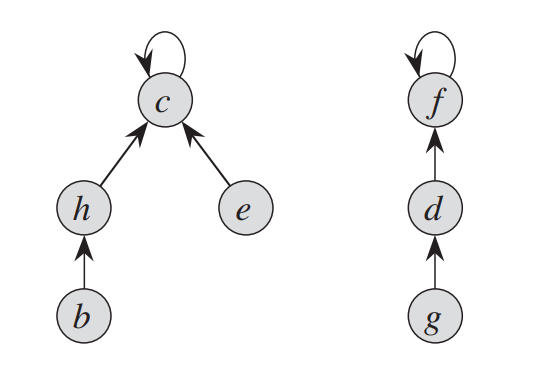
\includegraphics[scale=0.4]{media/ufds1}
\caption{A Disjoint Forest}
\end{figure}

The disjoint-set forest above represents the two sets $\{c, h, b, e\}$ with representative $c$ and $\{f, d, g\}$ with representative $f$. Note that the parent of any representative is itself. \\

How do we keep track of the parent of each vertex? This is easy --- we can just include an array called \verb!parent! as a part of our data structure implementation. For any vertex $v$, we can store the parent of $v$ in \verb!parent[v]!. \\

Now, we will discuss two heuristics to improve the running-time of various union-find operations. The first heuristic, known as the \vocab{union by rank heuristic}, is a heuristic that is applied when performing the \verb!UNION! operation. In particular, this heuristic specifies to make the root of the tree with fewer nodes to point to the root of the tree with more nodes.  Why? Because following the union by rank heuristic minimizes the overall depth of the resulting tree. \\


The following diagram illustrates the resulting tree that comes from performing the \verb!UNION! operation on two elements in the disjoint sets from the previous figure:
\newpage

\begin{figure}[h]
\centering
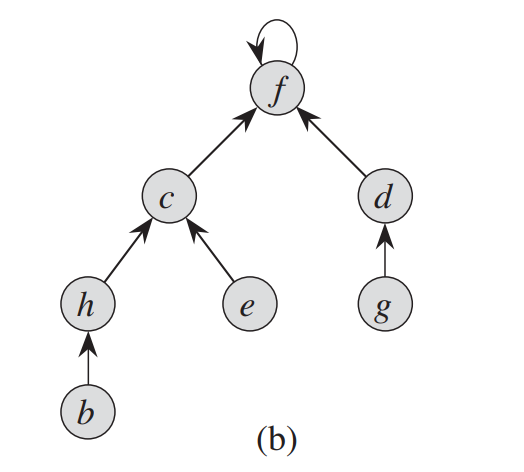
\includegraphics[scale=0.4]{media/ufds2}
\caption{Our Disjoint Forest after performing \texttt{UNION}}
\end{figure}

Note that $f$ is the representative of the resulting tree since we make the tree with fewer nodes point to the root of the tree with more nodes. \\

It would be computationally expensive to keep on recomputing the number of roots in each tree whenever we perform a \verb!UNION! operation. Thus, we can instead just maintain an array \verb!rank! which stores an upper bound on the height of each node. During a \verb!UNION! operation, we simply make the root with a smaller rank point to the root with the larger rank. \\


The second heuristic, known as \vocab{path compression} is a heuristic that is used during \verb!FIND-SET! operations to make each node on the find path point directly to the root. This technique is fairly easy to implement, and its purpose is to keep the depth of the tree small. \\


A C++ implementation of the union-find data structure is presented below:


\begin{lstlisting}
/* An implementation of the union-find data structure. */
class UnionFind {
    private:
        vector<int> parent;
        vector<int> rank;
    public:
        /* A constructor to initialize a union-find data structure with capacity N. */
        UnionFind(int N) {
            parent.assign(N, 0);
            rank.assign(N, 0);
            
            /* Each vertex is initially its own parent. */
            for (int i = 0; i < N; i++) {
                parent[i] = i;
            }
        }
    
    /* findSet(u) returns the representative of the set that u belongs to. */    
    int findSet(int u) {
        if (parent[u] == u) {
            /* u is the representative of its set. */
            return u;
        }
        /* Path compression heuristic. */
        parent[u] = findSet(parent[u]);
    }
    
    /* inSameSet(u, v) returns true if u and v are in the same set; false otherwise. */
    bool inSameSet(int u, int v) {
        /* We compare the set representatives. */
        return findSet(u) == findSet(v);
    }
    
    /* Union the sets that u and v belong in. */
    void unionSet(int u, int v) {
        if (!inSameSet(u, v)) {
            int rep1 = findSet(u);
            int rep2 = findSet(v);
            /* Union by rank heuristic. */
            if (rank[rep1] > rank[rep2]) {
                parent[rep2] = rep1;    
            } else {
                parent[rep1] = rep2;
                if (rank[rep1] == rank[rep2]) {
                    rank[rep2]++;
                }
            }
        }
    }

};
\end{lstlisting}


\subsection{Analysis of Union-Find Operations}

We won't derive 



\subsection{The Minimum Spanning Tree Problem}

The \vocab{minimum spanning tree} problem is stated below:




\subsubsection{Kruskal's Algorithm}

First, we'll discuss Kruskal's algorithm, which works by repeatedly finding a safe edge to add to the growing forest. In particular, this algorithm works by As stated in CLRS, ``Kruskal's algorithm qualifies as a greedy algorithm because, at each step, it adds to the forest an edge of least possible weight." \\

A 
\iffalse
\section{Thursday, February 20, 2020}

\subsection{Scheduling}


\subsection{Caching}

A \vocab{cache} is a piece of hardware or software that stores data in a special location so that future requests for that data can be served in a high-speed manner. The idea of caching is to store frequently-used values in a special area so that we can access the values in a quick manner. If a value is \textit{not} cached, then we say that the value is stored in \vocab{main memory}. 
\fi
\newpage
\section{Tuesday, February 25, 2020}


\subsection{Prefix Codes}

One particular class of encoding schemes are \vocab{prefix codes}. A prefix code for a set $S$ of letters is a function $\gamma$ that maps each letter $x\in S$ to some sequence of zeros and ones in such a way that for any $x, y \in S$ with $x \neq y$, the sequence $\gamma(x)$ is not a prefix of the sequence $\gamma(y)$. Why do many encoding schemes fall into this class? Because it removes ambiguity: --- if there exists a pair of letters where the bit string that encodes one letter is a prefix of the bit string that encodes the other, then there might be multiple interpretations of the same string.  \\

The ambiguity of encoding schemes that aren't prefix codes is demonstrated through the following example:

\begin{example}
[Ambiguity Morse Code] In Morse code, we typically encode letters with dashes and dots. For our purpose, we can think of dots and dashes as zeros and ones. Suppose $e$ maps to $0$ (a single dot), $t$ maps to $1$, and $a$ maps to $01$. Then the string $0101$ can have several interpretations: it can mean $eta, aa, etet$, or $aet$. If the morse code were a prefix code, then this problem wouldn't be present.
\end{example}


Now, here's an example illustrating the ease of using a prefix code:

\begin{example}
[Prefix Code Example] Suppose we have a set $S = \{a, b, c, d, e\}$ with the encoding $\gamma(a) = 11, \gamma(b) = 01, \gamma(c) = 001, \gamma(d) = 10, \gamma(e) = 000$. This defines a prefix code since no encoding is a prefix of any other. The string $cecab$ is encoded as $0010000011101$, and a recipient of this message can decipher this message to our single unique message.
\end{example}

In order to efficiently decipher a prefix code, we need an effective way to represent the prefix code so that we can easily pick off the codeword. This is typically done with a binary tree in which the leaves of the tree store the characters of our alphabet. How does this work? We interpret the binary codeword for a character as a simple path from the root to that character; the bit $0$ tells us to go to the left child, whereas the bit $1$ tells us to go to the right child. \\

The following binary search tree illustrates a prefix code representation:

\begin{figure}[h]
\centering
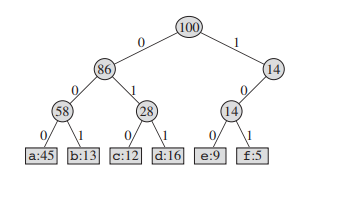
\includegraphics[scale=1]{media/prefix}
\caption{Prefix Code Representation}
\end{figure}

If we had the sequence $001011101$, then we could start at the root, and we'd scan our sequence from left to right. First, we counter two zeros, so we go to the left twice. At this point, we'd be at the vertex labelled $58$. Next, we encounter a $1$, so we go to the right. Thus, we obtain the character $b$. Next, we start at the root again, and we follow our procedure again. The next character that we decipher is $d$. This process continues until there are no more bits to process. \\


Given a tree $T$ corresponding to a prefix code, we can now easily compute the number of bits required to encode a file. In particular, for each character $c$ in our alphabet $S$, we can let $\verb!freq[c]!$ denote the frequency of $c$ in our file. Moreover, we can let $d_{T}(c)$ denote the depth of $c$'s leaf in the tree. With this notation, the number of bits required to encode a file is given by 
\[
\sum_{c \in S} \verb!freq[c]! \cdot d_{T}(c).
\]

We call this the \vocab{cost} of the tree $T$. 

\subsubsection{Constructing a Huffman code}

Now that we've introduced prefix codes, we'll talk about an optimal prefix code known as a \vocab{Huffman code}, whose tree representation has minimum cost. The algorithm constructing the tree is presented below: \\

\newpage

\vspace{1em}
\begin{center}
\line(1,0){400}
\end{center}

\begin{allintypewriter}
\# Input: A set C representing the set of all possible characters that 

\# might appear in our text, and an array freq[] in which freq[k] represents 

\# the frequency of the character k in our text.

\# Output: The root of a binary representing our encoding minimum cost.

\hspace{0cm}

HUFFMAN(C, freq) \string{

\hspace{0.5cm} let Q be a minimum priority queue

\hspace{0.5cm} for each element c in C \string{ enqueue c into Q \string }

\hspace{0cm}

\hspace{0.5cm} for i = 1 to n - 1 \string{

\hspace{1cm} let z be a new node

\hspace{1cm} x = EXTRACT-MIN(Q)

\hspace{1cm} y = EXTRACT-MIN(Q)

\hspace{1cm} z.left = x

\hspace{1cm} z.right = y

\hspace{1cm} \verb!freq[z] = freq[x] + freq[y]!

\hspace{1cm} insert z into Q.

\hspace{0.5cm} \string}

\hspace{0.5cm} return EXTRACT-MIN(Q) /* Return the root of the tree. */

\string}

\begin{center}
\line(1,0){400}
\end{center}
\end{allintypewriter}

How does this algorithm work?

\begin{enumerate}
    \item Firstly, we enqueue all of the characters in $C$ into our minimum priorty queue $Q$.
    \item The for-loop repeatedly extracts the two vertices with the lowest frequency and replaces them in the queue with a new node representing their ``merger" (parent). The frequency of $z$ is the sum of the frequencies of $x$ and $y$.
    \item After $n - 1$ merges, there's only one node left in the queue, which is the root of the code tree.
\end{enumerate}

If we're using a binary heap, then the algorithm runs in $\mathcal{O}(n\log(n))$ time since we perform $\mathcal{O}(n)$ calls to \verb!EXTRACT-MIN!, which is an $\mathcal{O}(\log(n))$ operation.


While we won't show it, it can be shown that this construction of a tree is optimal. This procedure counts as a greedy algorithm since, at each step, we greedily extract the characters with the lowest frequency.


\subsection{Matrix Multiplication}

The next problem we'll discuss is stated as follows:

\begin{quote}
    Given two $n\times n$ matrices $A$ and $B$, compute the $n \times n$ matrix $C$ whose $(i, j)^{\text{th}}$ entry is defined by $c_{ij} = \sum_{k=1}^{n}a_{ik} b_{kj}$. In other words, we want to compute the product $C = AB$. 
\end{quote}

The brute force solution is $\mathcal{O}(n^3)$. In this algorithm, we just use three loops, and we compute each value $c_{ij}$ in $C$ as the summation provided in the problem statement. Of course, we want to do better. \\

Another idea is to perform a divide-and-conquer technique on the matrix. In particular, we can divide the matrix into four submatrices (top left corner, top right corner, bottom left corner, bottom right corner), and we can calculate the products recursively. The time complexity of this algorithm is given by the recurrence $T(n) = 8T(n/2) + \mathcal{O}(n^2)$. Unfortunately, by Master's Theorem, we know that the solution to this recurrence will be $\mathcal{O}(n^3)$, which isn't any better. 
\newpage
\section{Thursday, February 27, 2020}
Last time, we introduced the matrix multiplication problem whose brute force solution runs in $\O(n^3)$ time. Today, we'll introduce \vocab{Strassen's algorithm}, a quicker solution to the matrix multiplication problem.


\subsection{Strassen's Algorithm}

Suppose we want to compute the matrix product $\mathbf{C} = \mathbf{A}\mathbf{B}$. Strasen's algorithm is a divide-and-conquer algorithm that works by partitioning the three matrices $\mathbf{A}, \mathbf{B}$, and $\mathbf{C}$ into equally sized block matrices as follows: \\

\[
\mathbf{A} = \begin{pmatrix}
\mathbf{A}_{1,1} & \mathbf{A}_{1,2} \\
\mathbf{A}_{2, 1} & \mathbf{A}_{2,2}
\end{pmatrix} \hspace{1cm} 
\mathbf{B} = \begin{pmatrix}
\mathbf{B}_{1,1} & \mathbf{B}_{1,2} \\
\mathbf{B}_{2, 1} & \mathbf{B}_{2,2}
\end{pmatrix} \hspace{1cm} 
\mathbf{C} = \begin{pmatrix}
\mathbf{C}_{1,1} & \mathbf{C}_{1,2} \\
\mathbf{C}_{2, 1} & \mathbf{C}_{2,2}
\end{pmatrix} 
\]


Our naive algorithm would compute the following quantities:

\begin{enumerate}
    \item $\mathbf{C}_{1,1} = \mathbf{A}_{1,1} \mathbf{B}_{1,1} + \mathbf{A}_{1,2}\mathbf{B}_{2,1}$, 
    \item $\mathbf{C}_{1,2} = \mathbf{A}_{1,1} \mathbf{B}_{1,2} + \mathbf{A}_{1,2}\mathbf{B}_{2,2}$, 
    \item $\mathbf{C}_{2,1} = \mathbf{A}_{2,1} \mathbf{B}_{1,1} + \mathbf{A}_{2,2}\mathbf{B}_{2,1}$, 
    \item $\mathbf{C}_{2,2} = \mathbf{A}_{2,1} \mathbf{B}_{1,2} + \mathbf{A}_{2,2}\mathbf{B}_{2,2}$, 
\end{enumerate}


With this construction, however, we require $8$ total multiplications to calculate our matrix. Strassen's algorithm works by cleverly rewriting some of these expressions so that we only require $7$ multiplications (similar to how Karatsuba's algorithm for large-integer multiplication). More precisely, we define the following matrices:

\begin{enumerate}
    \item $\mathbf{M}_{1} \defeq (\mathbf{A}_{1,1} + \mathbf{A}_{2,2})(\mathbf{B}_{1,1} + \mathbf{B}_{2,2})$,
    \item $\mathbf{M}_{2} \defeq (\mathbf{A}_{2,1} + \mathbf{A}_{2,2})\mathbf{B}_{1,1}$, 
    \item $\mathbf{M}_{3} \defeq \mathbf{A}_{1,1}(\mathbf{B}_{1,2} - \mathbf{B}_{2,2})$,
    \item $\mathbf{M}_{4} \defeq \mathbf{A}_{2,2}(\mathbf{B}_{2,1} - \mathbf{B}_{1,1})$,
    \item $\mathbf{M}_{5} \defeq (\mathbf{A}_{1,1} + \mathbf{A}_{1,2})\mathbf{B}_{2,2}$
    \item $\mathbf{M}_{6} \defeq (\mathbf{A}_{2,1} - \mathbf{A}_{1,1})(\mathbf{B}_{1,1} + \mathbf{B}_{1,2})$,
    \item $\mathbf{M}_{7} \defeq (\mathbf{A}_{1,2} - \mathbf{A}_{2,2})(\mathbf{B}_{2,1} + \mathbf{B}_{2,2})$.
\end{enumerate}

Note that computing the values of these matrices requires only $7$ multiplications (one for each $M_{k})$ instead of the usual $8$. We can now express our block matrices in terms of the $M_{k}$ matrices as follows:

\begin{enumerate}
    \item $\mathbf{C}_{1,1} = \mathbf{M}_{1} + \mathbf{M}_{4} - \mathbf{M}_{5} + \mathbf{M}_{7}$,
    \item $\mathbf{C}_{1,2} = \mathbf{M}_{3} + \mathbf{M}_{5}$,
    \item $\mathbf{C}_{2,1} = \mathbf{M}_{2} + \mathbf{M}_{4}$
    \item $\mathbf{C}_{2,2} = \mathbf{M}_{1} - \mathbf{M}_{2} + \mathbf{M}_{3} + \mathbf{M}_{6}$.
\end{enumerate}


We can iterate the procedure of dividing our matrices into blocks recursively until the submatrices are just numbers. \\

How fast does Strassen's algorithm run? Let $f(n)$ denote the number of multiplication operations we perform on a $2^{n}\times 2^{n}$ matrix. By the recursive application of Strassen's algorithm, we find $f(n) = 7f(n - 1) + c4^{n}$, where $c$ is some positive constant that depends on the number of additions performed at each step of the operation. Thus, we find $f(n) = (7 + o(1))^{n}$. Letting $N = 2^{n}$, we conclude that Strassen's algorithm runs in $\mathcal{O}(N^{\log_{2}(7) + o(1)})  \approx \mathcal{O}(N^{2.8074})$ time. \\


\subsection{Closest Pair of Points}

The closest pair of points problem is stated as follows:

\begin{quote}
    Given $n$ points in the plane $P = \{p_1, p_2, p_3, \ldots, p_n\}$, find two points $p_i$ and $p_j$ such that the Euclidean distance between $p_i$ and $p_j$ is minimal. 
\end{quote}

A simple brute force solution is to consider all ${n\choose 2}$ pairs of points, and keep track of the minimum distance value seen so far (this \verb!minimum! variable would initially be set to $\infty$). The runtime of this algorithm is $\mtahcal{O}(n^2)$ since computing the distance between two points is a constant-time operation. \\

Next class, we'll present a more efficient solution. 

% March
\newpage
% \iffalse
\section{Tuesday, March 3, 2020}

Recall the closest pair of points problem:

\begin{quote}
    Given $n$ points in the plane, find the pair whose Euclidean distance is minimal.
\end{quote}

Last time, we discussed a brute force $\mathcal{O}(n^2)$ solution to this problem. Today, we'll see a more efficient 

\subsection{Closest Pair of Points}
x

\subsection{Fast Fourier Transforms}


\newpage
\section{Thursday, March 5, 2020}

Today, we'll begin discussing our last divide-and-conquer topic: the Fast Fourier (``four-ee-aye") Transform. The problem that we are trying to solve is stated as follows:

\begin{quote}
    Given two vectors $a = (a_0, a_1, \ldots, a_{n - 1})$ and $b = (b_0, b_1, \ldots, b_{n - 1})$, compute the convolution $a\star b$ of $a$ and $b$. 
\end{quote}

Before discussing the algorithm that lets us do this, let's first discuss convolutions and why they're important. 

\subsection{Convolutions}

A \vocab{convolution} of two vectors $a$ and $b$ is a method of ``combining" the two vectors. More precisely, we define the convolution of the vectors $a = (a_0, a_1, \ldots, a_{n - 1})$ and $b = (b_0, b_1, \ldots, b_{n - 1})$ by the vector $c = (c_0, c_2, \ldots, c_{2n - 2})$ in which

\[
c_k = \sum_{(i, j) \mid i + j = k} a_i b_j.
\]

In other words, we have,

\[
a\star b = (a_0b_0, a_0b_1 + a_1b_0, \ldots, a_{n-1}b_{n-1}).
\]

Note that each summand in the $k^{\text{th}}$ component of this vector exhausts all possible pairs of indices that sum to $k$. Moreover, note that the convolution of two $n$-dimensional vectors produces a $(2n - 1)$-dimensional vector. However, unlike the vector sum and inner product, the convolution can easily be generalized to vectors of different lengths: if $a = (a_0, a_1, \ldots, a_{m - 1})$ and $b = (b_0, b_1, \ldots, b_{n - 1})$, then we define $a \star b$ to be a vector with $m + n - 1$ coordinates, where the $k^{\text{th}}$ coordinate is equal to the sum over all $a_ib_j$ in which $i + j = k$, $i < m$ and $b < n$. \\[1em]


Why do we care about the convolution? Here are some examples in which convolutions are useful:

\begin{example}
[Polynomial Multiplication]
Suppose we have two polynomials $A(x) = a_0 + a_1x + a_2x^2 + \cdots + a_{m - 1}x^{m - 1}$ and $B(x) = b_0 + b_1x + b_2x^2 + \cdots + b_{n - 1}x^{n - 1}$ and we wish to compute the product $C(x) = A(x) \cdot B(x)$. In order to do so, we can define the vectors $a = (a_0, a_1, \ldots, a_{m - 1})$ and $b = (b_0, b_1, \ldots, b_{n - 1})$ and compute the convolution $c = a\star b$. In the polynomial $C(x)$, the coefficient of $x^{k}$ is equal to the $k^{\text{th}}$ component of $c$.
\end{example}


\begin{example}
[Combining Histograms]
Suppose we're studying a population of people, and we have two histograms. The first histogram shows the annual income of all the men in the population, and the other shows the annual income of all the women. We would like to produce a new histogram showing for each $k$ the number of pairs $(M, W)$ for which man $M$ and woman $W$ have a combined income of $k$. This problem can be restated as a convolution. More precisely, let $a = (a_0, \ldots, a_{m - 1})$ and $b = (b_0, \ldots, b_{n - 1})$ be our histograms, and let $c_k$ denote the number of $(m, w)$ pairs with combined income $k$. Observe that $c_k$ is the number of ways to choose a man with income $a_i$ and woman with income $b_j$ with $i + j = k$. This quantity is given by a convolution.
\end{example}

\begin{example}
[Sum of Independent Random Variables]
If one is familiar with probability theory, then they may have encountered a theorem which tells us that the probabiliy distribution function for the sum of two random variables is a convolution of the distributions of the summands.
\end{example}

Now that we've motivated the importance of convolutions, we'll now discuss how to compute convolutions efficiently. For simplicity, we consider the case in which our two vectors have equal length (i.e. $m = n)$; however, our results hold for vectors of unequal length. \\

Computing a convolution efficiently is more difficult than it seems. If, for each $k$, we just calculate the sum $\sum_{(i, j) \mid i + j = k} a_ib_j$ and use it as the $k^{\text{th}}$ coordinate in our convolution vector, we end up with an $\mathcal{O}(n^2)$ algorithm. Fortunately, we can do better --- the \vocab{fast Fourier Transform} allows us to compute convolutions in $\mathcal{O}(n\log(n))$ time.

\subsection{The Fast Fourier Transform}

In order to compute convolutions quickly, we will make use of the connection between the convolution and polynomial multiplication. However, rather than using convolutions to perform polynomial multiplication, we will exploit the connection in the opposite direction. \\


Given two vectors $a = (a_0, \ldots, a_{n - 1})$ and $b = (b_0, \ldots, b_{n - 1})$, we define $A(x)$ and $B(x)$ to be the polynomials $a_0 + a_1x + \cdots + a_{n-1}x^{n-1}$ and $b_0 + b_1x + \cdots + b_{n-1}x^{n-1}$, respectively. Under this interpretation, we wish to compute the product $C(x) = A(x)B(x)$ in $\mathcal{O}(n\log(n))$ time. From there, we can simply ``read off" the convolution directly from the coefficients of $C(x)$. \\

Now, instead of multiplying $A$ and $B$ directly, we can treat them as functions of the variable $x$ and multiply them with the following three steps:

\begin{enumerate}
    \item Choose $2n$ values $x_1, x_2, \ldots, x_{2n}$ and evaluate $A(x_j)$ and $B(x_j)$ for each $j = 1, 2, \ldots, 2n$.
    \item Now for each index $1 \leq j \leq 2n$, we can easily compute $C(x_j)$. In particular, $C(x_j)$ is equal to the product of the two numbers $A(x_j)$ and $B(x_j)$.
    \item Finally, we need to recover the polynomial $C$ from its values on $x_1, x_2, \ldots, x_{2n}$. Since any polynomial of degree $d$ is fully determined by a set of $d + 1$ or more points, this is clearly possible. Since each $A$ and $B$ have degree at most $n - 1$, their product $C$ has degree at most $2n - 2$. Thus, it can be reconstructed from the values $C(x_1), C(x_2), \ldots, C(x_{2n})$ that we computed earlier.
\end{enumerate}

This approach to multiplying polynomials sounds promising, but there are a couple of issues we need to address. Evaluating the polynomials $A$ and $B$ on a single point takes $\Omega(n)$ operations (using Horner's method\footnote{\url{https://en.wikipedia.org/wiki/Horner\%27s_method}}, and our plan calls for performing $2n$ such evaluations. This brings us back up to quadratic time immediately. Moreover, we need a way to quickly reconstruct the polynomial $C$ from the points $C(x_1), C(x_2), \ldots, C(x_2n)$. \\

We address these two issues separately.

\subsubsection{Polynomial Evaluation}

We need to evaluate the polynomials $A$ and $B$ on $2n$ different points quickly. The key idea to doing this quickly is to find a set of $2n$ points $x_1, \ldots, x_{2n}$ that are related in some way so that the work in evaluating $A$ and $B$ on all of them can be shared across different evaluations. A set that works very well for us is the roots of unity. \\

\begin{definition}
An \vocab{$n^{\text{th}}$ root of unity} is a number $z$ satisfying the equation $z^{n} = 1$.
\end{definition}

It can be shown that there are $n$ $n^{\text{th}}$ roots of unity. Moreover, these roots are given by $e^{2k\pi i/n}$ for $k = 0, 1, \ldots, n - 1$. Clearly, each of these complex numbers satisfy our definition since
\[
(e^{2k \pi i/n})^{n} = e^{2k \pi i} = (e^{2 \pi i})^{k} = 1^{k} = 1.
\]

For our numbers $x_1, \ldots, x_{2n}$ on which to evaluate $A$ and $B$, we will choose the $(2n)^{\text{th}}$ roots of unity, and we propose a recursive procedure to compute $A$ on each of the $(2n)^{\text{th}}$ roots of unity. For simplicity, we henceforth assume that $n$ is a power of $2$. \\

Let $A_{\text{even}}(x)$ and $A_{\text{odd}}(x)$ be two polynomials that consist of the even and odd coefficients of $A$, respectively. That is, we have,
\[
A_{\text{even}}(x) = a_0 + a_2x + a_4x^2 + \cdots + a_{n - 2}x^{(n - 2)/2},
\]

and

\[
A_{\text{odd}}(x) = a_1 + a_3x + a_5x^2 + \cdots + a_{(n - 1)}x^{(n - 2)/2}.
\]

By simple algebra, we can see that we can express $A(x)$ as 

\[
A(x) = A_{\text{even}}(x^{2}) + xA_{\text{odd}}(x^{2}),
\]

which demonstrates that we can compute $A(x)$ in a constant number of operations provided that we already have $A_{\text{even}}$ and $A_{\text{odd}}$. Now suppose we evaluate both $A_{\text{even}}$ and $A_{\text{odd}}$ on the $n^{\text{th}}$ roots of unity. This is an exact replica of the problem we face with $A$ and the $(2n)^{\text{th}}$ roots of unity, except the input is half as large; the degrees of our two polynomials are $(n - 2)/2$ rather than $n - 1$. Moreover, we have $n$ roots of unity rather than $2n$. Thus, we can perform these evaluations recursively in time $T(n/2)$ for each of $A_{\text{even}}$ and $A_{\text{odd}}$, for a total of $2T(n/2)$ time. \\

But, how do we perform these evaluations? This can be done with $\mathcal{O}(n)$ additional operations given the results from the recursive calls on $A_{\text{even}}$ and $A_{\text{odd}}$.  Let $\omega = e^{2\pi i k/2n}$ be a $(2n)^{\text{th}}$ root of unity for some integer $k$. The quantity $\omega^{2}$ is equal to $e^{2\pi k i/n}$, which is an $n^{\text{th}}$ root of unity.  \\

Thus, when we go to compute $A(\omega) = A_{\text{even}}(\omega^{2}) + \omega \cdot A_{\text{odd}}(\omega^2)$,we find that both evaluations on the right-hand side have been performed in a recursive step, which means that we can compute $A(\omega)$ in a constant number of operations. Repeating for each of the $2n$ roots of unity is therefore $\mathcal{O}(n)$ additional operations. \\

Therefore, our bound $T(n)$ on the number of operations satisfies $T(n) = 2T(n/2) + \mathcal{O}(n)$, which gives us the desired $\mathcal{O}(n\log(n))$ bound for the first step of our algorithm. \\


\subsubsection{Polynomial Interpolation}

Next, we'll discuss how to Now, we've seen how to evaluate $A$ and $B$ on the set of all $(2n)^{\text{th}}$ roots of unity using $\mathcal{O}(n\log(n))$ operations. Also, we can clearly perform the second step of our algorithm naively in linear time. Thus, to conclude the algorithm for multiplying $A$ and $B$, we need to reconstruct the polynomial $C$ from its values on the $(2n)^{\text{th}}$ roots of unity in $\mathcal{O}(n\log(n))$ time. \\


The reconstruction of $C$ can be achieved by defining an appropriate polynomial and evaluating it at the $(2n)^{\text{th}}$ roots of unity. This is exactly what we've just seen how to do using $\mathcal{O}(n\log(n))$ operations, so we'll do it here again. This requires an additional $\mathcal{O}(n\log(n))$ operations, and it concludes our algorithm. \\

Consider a polynomial $C(x) = \sum_{s=0}^{2n - 1} c_sx^s$ that we want to reconstruct from its values at the $C(\omega_{s, 2n})$ at the $(2n)^{\text{th}}$ roots of unity. Define a new polynomial $D(x) \defeq \sum_{s = 0}^{2n - 1} d_{s}x^{s}$ where $d_s = C(\omega_{s, 2n}$. We now consider the values of $D(x)$ at the $(2n)^{\text{th}}$ roots of unity: 

\begin{align*}
D(\omega_{j, 2n}) &= \sum_{s = 0}^{2n - 1} C(\omega_{s, 2n}) \omega_{j, 2n}^{s} \\[1em]
&= \sum_{s=0}^{2n - 1}\left( \sum_{t = 0}^{2n - 1} c_{t} \omega_{s, 2n}^{t} \right)\omega_{j, 2n}^{s}. 
\end{align*}

Now since $\omega_{s, 2n} = (e^{2\pi i/2n})^{s}$, we get that 
\[ 
D(\omega_{j, 2n}) = \sum_{t=0}^{2n - 1}c_t \sum_{s = 0}^{2n - 1} \omega_{t + j, 2n}^{s}).
\]
However, note that for any $(2n)^{\text{th}}$ root of unity $\omega \neq 1$, we have $\sum_{s = 0}^{2n - 1} \omega^{s} = 0$. Thus, the only term that of the last line's outer sum that is not equal to $0$ is for $c_t$ such that $\omega_{t + j, 2n} = 1$. This happens precisely when $t + j = 2n - j$. \\

It follows immediately that for any polynomial $C(x) = \sum_{s = 0}^{2n - 1}c_sx^{s}$ and corresponding polynomial $D(x) = \sum_{s = 0}^{2n - 1} C(\omega_{s, 2n}) x^{s}$, we have $c_s = \frac{1}{2n} D(\omega_{2n - s, 2n})$.  \\

Thus, we can reconstruct the polynomial $C$ from its values on the $(2n)^{\text{th}}$ roots of unity, and the coefficients of $C$ are the coordinates in the convolution vector $a \star b$ that we were originally seeking. Therefore, we are done.
\iffalse
\newpage
\section{Thursday, March 12, 2020}

\subsection{All-Pairs Shortest Paths}

Suppose we are given a weighted, directed graph $G = (V, E)$ with a weight function $w : E \rightarrow \mathbb{R}$ that maps edges to real-valued weights (the mapped values are henceforth referred to as \vocab{edge weights}). Moreover, for any two vertices $u, v\in V$, we define $\delta(u, v)$ as the \vocab{shortest path} (where we minimize the sum of edge weights) between the vertices $u$ and $v$. \\

We want to find, for every pair of vertices $u, v \in V$, the value of $\delta(u, v)$. This is known as the \vocab{all-pairs shortest path problem} (ASSP). Note that this differs from the single-source shortest path problem (SSSP) (which Dijkstra's algorithm solves) since SSSP only wants to compute the shortest path from a single source to a single destination. On the other hand, ASSP wants to compute the distances between \textit{all} pairs of vertices. \\

We can solve the ASSP by running a single-source shortest path algorithm $|V|$ times (once for each possible source vertex). Using a binary min-heap implementation of the minimum priority queue in Dijkstra's algorithm yields a running time of $\mathcal{O}(VE\log(V))$. However, Dijkstra's algorithm has a disadvantage: it doesn't work for negative edge weights. If $G$ has negative edge weights, then we need to use a different SSSP algorithm, like Bellman-Ford, which would increase our running time to $\mathcal{O}(V^4).$ Thus, we seek to do better.


\subsubsection{Floyd-Warshall Algorithm}

The \vocab{Floyd-Warshall algorithm} solves ASPS by 

\subsubsection{Transitive Closure}

asdf

\fi
% April
\newpage
\section{Tuesday, April 7, 2020} 

\subsection{Subset Sum Problem}

Today, we'll discuss another classical dynamic programming problem, known as the \vocab{subset sum problem}.\footnote{The subset sum problem is a special case of another classical dynamic programming problem, known as the \vocab{knapsack problem}. In the knapsack problem, each item $1 \leq i \leq n$ has a value $v_i$ and weight $w_i$. For each item, we want to assign a number $x_i \in \{0, 1\}$ so that $\sum_{i}x_iv_i$ is maximized subject to $\sum_{i} x_i w_i \leq W$. } The subset problem is stated as follows:

\begin{quote}
    Suppose we are given $n$ items $\{1, 2, \ldots, n\}$ each with nonnegative weight $w_i$. We are also given a bound $W$. How do we select a subset $S$ of the items so that $\sum_{i\in S} w_i$ is maximized subject to $\sum_{i\in S} w_i \leq W$?
\end{quote}

In other words, given $n$ items each with nonnegative weights, what's the closest we can get to a weight of $W$ without going over?  \\

\begin{example}
[Subset Sum Example] Suppose $n = 3$ with $w_1 = 2$, $w_2 = 3$, $w_3 = 4$, and $W = 5$. The solution to this instance of the subset problem is $\boxed{5}$ --- it is optimal to choose $w_1$ and $w_2$. 
\label{greedy:01}
\end{example}

Does a greedy solution work? One greedy rule might be to sort the items in ascending order by weight and always pick the item with maximal weight that hasn't been taken yet. However, this greedy rule fails in \Cref{greedy:01}; we'll end up with a total weight of $4$, which is sub-optimal. \\

We demonstrate how we can use dynamic programming to solve this problem. Recall that the main principles of dynamic programming are to come up with a recurrence so that we can relate the problem we want to solve to ``smaller" subproblems. The tricky issue is determining what a good set of subproblems consists of. \\

One general strategy in dynamic programming is to consider subproblems consisting of only the first $i$ ``requests," or items. We can use this strategy here. Formally, let $\OPT(i)$ denote the best possible solution using only the subset $\{1, \ldots, i\}$ of the original set of items. Now, the key to this problem is to concentrate on an optimal solution and consider two different cases, depending on whether or not the last item $n$ we processed is part of this optimum solution or not. Let $\mathcal{O}$ denote an optimal solution.\\


If $n \not \in \mathcal{O}$, then $\OPT(n) = \OPT(n - 1)$. This is obvious --- if the last item we processed isn't a part of our optimal solution, then the optimal solution using only $\{1, 2, \ldots, n - 1\}$ shouldn't change when $n$ is included (we now have the option to take $n$, but we don't want $n$ anyways!). \\


The only other case we have to consider is the case in which $n \in \mathcal{O}$. What we need to find is a simple recursion that tells us the best possible value we can obtain for solutions containing the last request $n$. Note that accepting request $n$ does not immediately imply that we have to reject any other requests. Instead, it means that for the subset of requests $S \subseteq \{1, 2, \ldots, n - 1\}$ that we will accept, we have less available weight left. More precisely, we will have $W - w_n$ weight left for the remaining set of items we accept. \\


This suggests that we need more subproblems: we cannot just use the value $\OPT(n - 1)$ when we're including item $n$ since the combined weight of the items in $\OPT(n - 1)$ and item $n$ might exceed $W$. What we precisely need is the best solution using the first $n - 1$ items when the total weight allowed is $W - w_n$. Thus, we require many more subproblems: one for each initial set $\{1, 2, \ldots, i\}$ of the items, and each possible value for the remaining weight available $w$. \\

More precisely, if each of our items $1, 2, \ldots, n$ have integer weights $w_i$ and our maximum weight bound is $W$, then we have a subproblem for each $i = 0, 1, \ldots, n$ and each integer $0 \leq w \leq W.$ We henceforth use $\OPT(i, w)$ to denote the value of the optimal solution using the subset of the items $\{1, 2, \ldots, i\}$ with maximum allowed weight $w$. That is,

\[
\OPT(i, w) = \max_{S \subseteq \{1, 2, \ldots, i\}} \sum_{j \in S} w_j \hspace{1em} \text{subject to  } \sum_{j \in S} w_j \leq w.
\]

Using this new set of subproblems, we can note that the final answer we want is $\OPT(n, W)$. Moreover, we can express the value $\OPT(i, w)$ as an expression from smaller problems. These results are summarized below:

\begin{enumerate}
    \item If $n \not \in \O$, then $\OPT(n, W) = \OPT(n - 1, W)$ since we can ignore the item $n$.
    \item If $n\in \O$, then $\OPT(n, W) = w_n + \OPT(n - 1, W - w_n)$ since we now want to use the remaining capacity $W - w_n$ in an optimal way across the first $n - 1$ items.
\end{enumerate}

If $W < w_n$ for some item $n$, then we require $\OPT(n, W) = \OPT(n - 1, W)$ since we aren't allowed to take item $n$ due to our constraint. Now that we've considered both cases, we can get the optimum solution by simply taking the better of these two options. Therefore, we obtain the following recurrence:

\[
\OPT(i, W) = \begin{cases}
\max(\OPT(i - 1, w), w_i + \OPT(i - 1, W - w_i)) & \text{ if } w_i \leq W \\[1em]
\OPT(i - 1, w) & \text{ otherwise.}
\end{cases}
\]

Also, we have the base cases $\OPT(i, w) = 0$ provided that $i = 0$ since we aren't allowed to take any items when $i = 0$. \\

With our recurrence and base cases established, we are done. 


\end{document}